\documentclass[aspectratio=169,12pt]{beamer}

% ---------------------------------------------------------------
% Slides para projetar as quest\~oes do Bloco 7 (fazer em sala).
% Mesma identidade dos outros documentos de trabalho e energia:
% Palatino, versalete, uma cor de destaque (bord\^o).
% Os n\'umeros das quest\~oes s\~ao os mesmos da lista impressa.
% A ordem do deck \'e a do plano: primeiro o bloco ENEM/UTFPR,
% depois as de outras bancas, e por fim as duas de b\^onus.
% ---------------------------------------------------------------
\usepackage[utf8]{inputenc}
\usepackage[T1]{fontenc}
\usepackage[brazil]{babel}
\usepackage[sc]{mathpazo}   % sem 'osf': algarismos alinhados leem melhor projetados
\usefonttheme{serif}
\usepackage{microtype}
\usepackage{amsmath}
\usepackage{amssymb}
\usepackage{xcolor}
\usepackage{tikz}
\usepackage{pgfplots}
\pgfplotsset{compat=1.18}
\usetikzlibrary{arrows.meta, patterns, decorations.pathmorphing, positioning}
\graphicspath{{figuras/}}

\definecolor{vinho}{RGB}{122, 27, 42}
\definecolor{grafite}{RGB}{70, 70, 70}

\setbeamercolor{structure}{fg=vinho}
\setbeamercolor{normal text}{fg=black}
\setbeamercolor{alerted text}{fg=vinho}
\setbeamertemplate{navigation symbols}{}
\setbeamersize{text margin left=0.9cm, text margin right=0.9cm}

% ---------------------------------------------------------------
% T\'itulo de slide: versalete bord\^o \`a esquerda, fonte/tempo \`a
% direita, filete embaixo
% ---------------------------------------------------------------
\setbeamertemplate{frametitle}{%
  \vspace{0.18cm}%
  \begin{minipage}{\textwidth}
    {\large\scshape\color{vinho}\insertframetitle}%
    \hfill{\small\itshape\color{grafite}\insertframesubtitle}\\[-0.45em]
    {\color{vinho}\rule{\textwidth}{1.1pt}}
  \end{minipage}%
  \par\vspace{0.08cm}
}

\setbeamertemplate{footline}{%
  \hfill{\scriptsize\color{black!45}%
    trabalho e energia \,\textperiodcentered\, conserva\c{c}\~ao
    \,\textperiodcentered\, \insertframenumber}%
  \hspace{0.9cm}\vspace{0.25cm}%
}

% ---------------------------------------------------------------
% Alternativas
% ---------------------------------------------------------------
\newcommand{\optitem}[2]{%
  \par\hangindent=1.5em\hangafter=1
  \makebox[1.5em][l]{\textbf{#1)}}#2}

\newcommand{\alternativas}[5]{%
  \par\vspace{0.55em}%
  \begingroup\setlength{\parskip}{0.30em}%
  \optitem{a}{#1}\optitem{b}{#2}\optitem{c}{#3}\optitem{d}{#4}\optitem{e}{#5}%
  \par\endgroup}

% vers\~ao em duas colunas (a, b, c | d, e), para alternativas m\'edias
\newcommand{\alternativascols}[5]{%
  \par\vspace{0.5em}%
  \begingroup\setlength{\parskip}{0.28em}%
  \noindent
  \begin{minipage}[t]{0.48\textwidth}
    \optitem{a}{#1}\optitem{b}{#2}\optitem{c}{#3}
  \end{minipage}\hfill
  \begin{minipage}[t]{0.48\textwidth}
    \optitem{d}{#4}\optitem{e}{#5}
  \end{minipage}%
  \par\endgroup}

% vers\~ao em uma linha s\'o, para alternativas curtas (num\'ericas)
\newcommand{\alternativascurtas}[5]{%
  \par\vspace{0.7em}%
  \noindent\textbf{a)}~#1\hfill\textbf{b)}~#2\hfill\textbf{c)}~#3%
  \hfill\textbf{d)}~#4\hfill\textbf{e)}~#5\par}

% vers\~oes de quatro alternativas (estilo UERJ)
\newcommand{\alternativasquatro}[4]{%
  \par\vspace{0.55em}%
  \begingroup\setlength{\parskip}{0.30em}%
  \optitem{a}{#1}\optitem{b}{#2}\optitem{c}{#3}\optitem{d}{#4}%
  \par\endgroup}

\newcommand{\alternativascurtasquatro}[4]{%
  \par\vspace{0.7em}%
  \noindent\hspace*{0.06\textwidth}%
  \textbf{a)}~#1\hfill\textbf{b)}~#2\hfill\textbf{c)}~#3%
  \hfill\textbf{d)}~#4\hspace*{0.06\textwidth}\par}

% ---------------------------------------------------------------
% Slide de resposta (projetar depois de resolver no quadro)
% ---------------------------------------------------------------
\newcommand{\resposta}[2]{%
  \par\vspace{0.2em}
  {\Large\bfseries\color{vinho}Quest\~ao #1 \,\textemdash\, resposta: #2}
  \par\vspace{0.6em}}

\newcommand{\esquemaaula}{%
  {\scriptsize\itshape\color{grafite}(esquema da aula --- a prova n\~ao traz figura)}}

\setlength{\parskip}{0.35em}
\linespread{1.03}

% ---------------------------------------------------------------
\begin{document}
% ---------------------------------------------------------------

% ===================================================================
% CAPA
% ===================================================================
\begin{frame}[plain]
\vspace{0.6cm}
{\scshape\color{vinho}cursinho solid\'ario \,\textperiodcentered\, f\'isica}\\[-0.5em]
{\color{vinho}\rule{\textwidth}{1.6pt}}\\[1.0em]
{\huge\bfseries Quest\~oes em Sala}\\[0.45em]
{\LARGE Trabalho e Energia}\\[1.0em]
\hfill {\color{grafite}2026}\\[-0.3em]
{\color{black!30}\rule{\textwidth}{0.5pt}}\\[0.8em]
\end{frame}

% ===================================================================
% ROTEIRO
% ===================================================================
\begin{frame}
\frametitle{Roteiro}
\framesubtitle{35 min}

\footnotesize
{\renewcommand{\arraystretch}{1.10}
\begin{tabular}{@{}clll@{}}
  \textbf{\#} & \textbf{Fonte} & \textbf{O que cobra} & \textbf{Tempo}\\[0.15em]
  \hline
  \rule{0pt}{1.15em}%
  Q8  & ENEM 2011          & Conserva\c{c}\~ao: salto com vara            & 3 min \\
  Q11 & ENEM 2018          & Energia el\'astica ($kx^2/2$)                & 4 min \\
  Q12 & ENEM 2022          & For\c{c}a m\'edia e energia dissipada        & 3 min \\
  Q15 & UTFPR Ver\~ao 2026 & Pot\^encia: $P = Fv$                         & 2 min \\
  Q17 & UTFPR Inverno 2023 & Rendimento e kWh (fotovoltaico)              & 5 min \\
  Q16 & ENEM 2016          & Pot\^encia da usina de Itaipu                & 4 min \\[0.35em]
  Q10 & UERJ               & Conserva\c{c}\~ao com conta                  & 4 min \\
  Q13 & UNIFOR CE          & Energia dissipada na queda                   & 4 min \\
  Q1  & UFF                & Sinal do trabalho e o \^angulo               & 2 min \\
  Q5  & FGV                & Teorema $W = \Delta E_c$                     & 4 min \\
\end{tabular}}

\vspace{0.5em}
{\footnotesize\color{grafite}\itshape
As seis primeiras s\~ao de ENEM e UTFPR, que \'e o que a turma vai
prestar. \textbf{B\^onus}, se sobrar tempo: Q18 (UTFPR Ver\~ao 2025) e
Q19 (ENEM 2015).}

\end{frame}

% ===================================================================
% BLOCO ENEM / UTFPR
% ===================================================================

% ===================================================================
% Q8 --- ENEM 2011
% ===================================================================
\begin{frame}
\frametitle{Quest\~ao 8}
\framesubtitle{ENEM 2011 \,\textperiodcentered\, $\sim$3 min}

\linespread{0.93}\selectfont
\begin{columns}[T]
\begin{column}{0.46\textwidth}
\small
Uma das modalidades presentes nas olimp\'iadas \'e o salto com vara. As
etapas de um dos saltos de um atleta est\~ao representadas na figura.

\vspace{0.5em}
Desprezando-se as for\c{c}as dissipativas, para que o salto atinja a
maior altura poss\'ivel, ou seja, o \textbf{m\'aximo de energia seja
conservada}, \'e necess\'ario que
\end{column}
\begin{column}{0.52\textwidth}
\centering
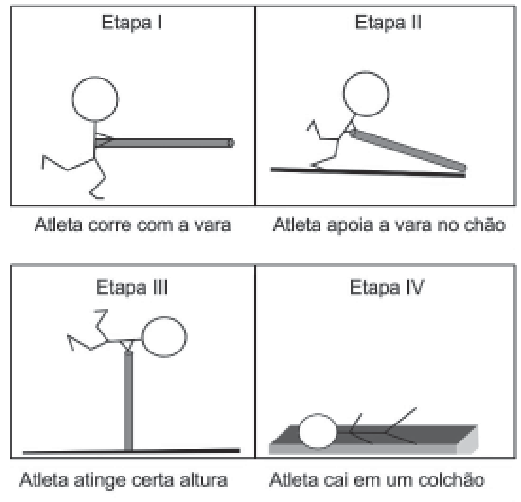
\includegraphics[height=4.0cm]{enem2011_q86_salto_vara}
\end{column}
\end{columns}

\vspace{-0.8em}
{\scriptsize
\alternativascols{a energia cin\'etica, representada na etapa I, seja
totalmente convertida em energia potencial el\'astica representada na
etapa IV.}%
{a energia cin\'etica, representada na etapa II, seja totalmente
convertida em energia potencial gravitacional, representada na
etapa IV.}%
{a energia cin\'etica, representada na etapa I, seja totalmente
convertida em energia potencial gravitacional, representada na
etapa III.}%
{a energia potencial gravitacional, representada na etapa II, seja
totalmente convertida em energia potencial el\'astica, representada na
etapa IV.}%
{a energia potencial gravitacional, representada na etapa I, seja
totalmente convertida em energia potencial el\'astica, representada na
etapa III.}}
\end{frame}

\begin{frame}
\frametitle{Quest\~ao 8}
\framesubtitle{gabarito}
\resposta{8}{C --- $E_c$ da etapa I vira $E_{pg}$ da etapa III}

A energia que faz o atleta subir \'e a \textbf{energia cin\'etica da
corrida} (etapa I). O ponto mais alto \'e a \textbf{etapa III}, onde
essa energia est\'a guardada como potencial gravitacional.

\vspace{0.4em}
\begin{center}
\begin{tikzpicture}[node distance=0.6cm]
  \node[draw=vinho, thick, rounded corners=3pt, inner sep=5pt]
    (a) {$E_c$ \ \scriptsize(etapa I: corrida)};
  \node[draw=black!45, rounded corners=3pt, inner sep=5pt,
        right=1.0cm of a] (b) {$E_{pe}$ \ \scriptsize(etapa II: vara)};
  \node[draw=vinho, thick, rounded corners=3pt, inner sep=5pt,
        right=1.0cm of b] (c) {$E_{pg}$ \ \scriptsize(etapa III: topo)};
  \draw[-{Stealth[length=3mm]}, thick] (a) -- (b);
  \draw[-{Stealth[length=3mm]}, thick] (b) -- (c);
\end{tikzpicture}
\end{center}

\vspace{0.3em}
{\color{grafite}\itshape A vara \'e s\'o o intermedi\'ario: guarda
energia el\'astica na etapa II e devolve em seguida. Na etapa IV ele
j\'a est\'a caindo --- por isso nenhuma alternativa que termina na
etapa IV pode estar certa.}
\end{frame}

% ===================================================================
% Q11 --- ENEM 2018
% ===================================================================
\begin{frame}
\frametitle{Quest\~ao 11}
\framesubtitle{ENEM 2018 \,\textperiodcentered\, $\sim$4 min}

\begin{columns}[T]
\begin{column}{0.58\textwidth}
\small
Um projetista deseja construir um brinquedo que lance um pequeno cubo
ao longo de um trilho horizontal, e o dispositivo precisa oferecer a
op\c{c}\~ao de mudar a velocidade de lan\c{c}amento. Para isso, ele
utiliza uma mola e um trilho onde o \textbf{atrito pode ser
desprezado}, conforme a figura.
\end{column}
\begin{column}{0.40\textwidth}
\centering
\vspace{0.4em}
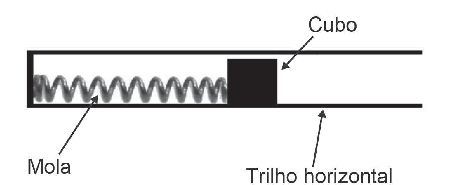
\includegraphics[height=2.2cm]{enem2018_q131_mola_trilho}
\end{column}
\end{columns}

\vspace{0.2em}
\small
Para que a velocidade de lan\c{c}amento do cubo seja \textbf{aumentada
quatro vezes}, o projetista deve

\vspace{-0.4em}
{\scriptsize
\alternativascols{manter a mesma mola e aumentar duas vezes a sua
deforma\c{c}\~ao.}%
{manter a mesma mola e aumentar quatro vezes a sua deforma\c{c}\~ao.}%
{manter a mesma mola e aumentar dezesseis vezes a sua
deforma\c{c}\~ao.}%
{trocar a mola por outra de constante el\'astica duas vezes maior e
manter a deforma\c{c}\~ao.}%
{trocar a mola por outra de constante el\'astica quatro vezes maior e
manter a deforma\c{c}\~ao.}}
\end{frame}

\begin{frame}
\frametitle{Quest\~ao 11}
\framesubtitle{gabarito}
\resposta{11}{B --- mesma mola, quatro vezes a deforma\c{c}\~ao}

\begin{columns}[T]
\begin{column}{0.52\textwidth}
Toda a energia da mola vira energia cin\'etica:
\[ \frac{k x^2}{2} = \frac{m v^2}{2}
   \;\Longrightarrow\; x = v\sqrt{\frac{m}{k}} \]

Com a \textbf{mesma} mola, $x$ \'e proporcional a $v$:
\[ v \to 4v \;\Longrightarrow\; x \to 4x \]
\end{column}
\begin{column}{0.44\textwidth}
\small
\textbf{E se trocasse a mola?}\\
Mantendo $x$, seria preciso
\[ k \to 16\,k \]
porque $v \propto \sqrt{k}$.

\vspace{0.5em}
{\color{grafite}\itshape As alternativas d) e e) s\~ao a pegadinha:
quem esquece o quadrado troca 16 por 2 ou 4.}
\end{column}
\end{columns}
\end{frame}

% ===================================================================
% Q12 --- ENEM 2022
% ===================================================================
\begin{frame}
\frametitle{Quest\~ao 12}
\framesubtitle{ENEM 2022 \,\textperiodcentered\, $\sim$3 min}

\footnotesize
Em um aut\'odromo, os carros podem derrapar em uma curva e bater na
parede de prote\c{c}\~ao. Para diminuir o impacto de uma batida,
pode-se colocar na parede uma \textbf{barreira de pneus}: isso faz com
que a colis\~ao seja mais demorada e o carro \textbf{retorne} com
velocidade reduzida. Outra op\c{c}\~ao \'e colocar uma \textbf{barreira
de blocos} de um material que se deforma, tornando-a t\~ao demorada
quanto a colis\~ao com os pneus, mas que \textbf{n\~ao permite a volta}
do carro ap\'os a colis\~ao.

\vspace{0.3em}
\small
Comparando as duas situa\c{c}\~oes, como ficam a for\c{c}a m\'edia
exercida sobre o carro e a energia mec\^anica dissipada?

\vspace{-0.3em}
{\scriptsize
\alternativascols{A for\c{c}a \'e maior na colis\~ao com a barreira de
pneus, e a energia dissipada \'e maior na colis\~ao com a barreira de
blocos.}%
{A for\c{c}a \'e maior na colis\~ao com a barreira de blocos, e a
energia dissipada \'e maior na colis\~ao com a barreira de pneus.}%
{A for\c{c}a \'e maior na colis\~ao com a barreira de blocos, e a
energia dissipada \'e a mesma nas duas situa\c{c}\~oes.}%
{A for\c{c}a \'e maior na colis\~ao com a barreira de pneus, e a
energia dissipada \'e maior na colis\~ao com a barreira de pneus.}%
{A for\c{c}a \'e maior na colis\~ao com a barreira de blocos, e a
energia dissipada \'e maior na colis\~ao com a barreira de blocos.}}
\end{frame}

\begin{frame}
\frametitle{Quest\~ao 12}
\framesubtitle{gabarito}
\resposta{12}{A --- for\c{c}a maior nos pneus, dissipa\c{c}\~ao nos blocos}

\linespread{0.92}\selectfont
\begin{columns}[T]
\begin{column}{0.48\textwidth}
\textbf{For\c{c}a --- o mesmo $\Delta t$}\\
Pneus: o carro \textbf{volta}, ent\~ao $\Delta v$ \'e maior
($v \to -v'$).

\vspace{0.2em}
Blocos: o carro \textbf{para}, $\Delta v$ \'e menor ($v \to 0$).

\vspace{0.2em}
No mesmo tempo, maior $\Delta v$ pede \textbf{maior for\c{c}a
m\'edia}: pneus.
\end{column}
\begin{column}{0.48\textwidth}
\textbf{Energia --- o que sumiu}\\
Blocos: o carro para, e \textbf{toda} a $E_c$ \'e dissipada.

\vspace{0.2em}
Pneus: ele sai com alguma velocidade, ent\~ao \textbf{sobra} energia
mec\^anica.

\vspace{0.2em}
Dissipa mais quem para: \textbf{blocos}.
\end{column}
\end{columns}

\vspace{0.4em}
{\color{grafite}\itshape\small As duas grandezas puxam para lados
diferentes, e \'e a\'i que a quest\~ao pega. Na vida real o pneu
protege porque \textbf{estica o tempo} --- mas aqui o enunciado j\'a
igualou os tempos de prop\'osito.}
\end{frame}

% ===================================================================
% Q15 --- UTFPR Ver\~ao 2026
% ===================================================================
\begin{frame}
\frametitle{Quest\~ao 15}
\framesubtitle{UTFPR Ver\~ao 2026 \,\textperiodcentered\, $\sim$2 min}

\begin{columns}[T]
\begin{column}{0.58\textwidth}
Uma caixa de 10 kg \'e i\c{c}ada por um guindaste com uma velocidade
constante de aproximadamente 5 m/s.

\vspace{0.4em}
Desconsiderando atritos e outras perdas e considerando
$g \approx 10$ m/s\textsuperscript{2}, assinale a alternativa com a
\textbf{pot\^encia m\'inima} do motor de i\c{c}amento necess\'aria
para realizar o i\c{c}amento descrito.
\end{column}
\begin{column}{0.40\textwidth}
\centering
\begin{tikzpicture}[scale=0.92]
  % ch\~ao
  \draw[thick] (-0.2,0) -- (4.0,0);
  \foreach \x in {-0.1,0.2,...,3.9}
    \draw[black!45] (\x,0) -- (\x-0.18,-0.18);
  % mastro, lan\c{c}a e escora
  \draw[line width=1.6pt, black!70] (0.6,0) -- (0.6,3.4);
  \draw[line width=1.6pt, black!70] (0.6,3.4) -- (3.0,3.4);
  \draw[thick, black!70] (0.6,2.7) -- (1.3,3.4);
  % cabo e gancho
  \draw[thick] (2.6,3.4) -- (2.6,2.15);
  \draw[thick] (2.5,2.15) -- (2.7,2.15);
  % caixa
  \draw[thick, fill=black!8] (2.05,1.45) rectangle (3.15,2.15);
  \node[font=\small] at (2.60,1.80) {10 kg};
  % velocidade
  \draw[-{Stealth[length=3mm]}, very thick, vinho] (3.45,1.45) -- (3.45,2.55)
    node[midway, right, font=\small] {$v = 5$ m/s};
\end{tikzpicture}\\[0.2em]
\esquemaaula
\end{column}
\end{columns}

\alternativascurtas{250 W}{500 W}{750 W}{1\,000 W}{1\,250 W}
\end{frame}

\begin{frame}
\frametitle{Quest\~ao 15}
\framesubtitle{gabarito}
\resposta{15}{B --- 500 W}

\begin{columns}[T]
\begin{column}{0.50\textwidth}
Velocidade \textbf{constante} $\Rightarrow$ a for\c{c}a do cabo
equilibra o peso:
\[ F = mg = 10\cdot 10 = 100\ \text{N} \]
\[ P = F v = 100\cdot 5 = \mathbf{500\ W} \]
\end{column}
\begin{column}{0.46\textwidth}
\textbf{Pelo outro caminho}\\
Em 1 s a caixa sobe 5 m e ganha
\[ mgh = 10\cdot 10\cdot 5 = 500\ \text{J} \]
ou seja, 500 J por segundo.
\end{column}
\end{columns}

\vspace{0.6em}
{\color{grafite}\itshape Estilo UTFPR: uma conta s\'o, direta. O
$P = Fv$ e o $P = W/\Delta t$ s\~ao a mesma coisa --- vale mostrar os
dois no quadro, porque a turma decora um e trava quando cai o outro.}
\end{frame}

% ===================================================================
% Q17 --- UTFPR Inverno 2023
% ===================================================================
\begin{frame}
\frametitle{Quest\~ao 17}
\framesubtitle{UTFPR Inverno 2023 \,\textperiodcentered\, $\sim$5 min}

\footnotesize\linespread{0.98}\selectfont
A energia solar \'e uma fonte renov\'avel e limpa que tem se tornado
cada vez mais importante. A instala\c{c}\~ao de sistemas fotovoltaicos
\'e uma das maneiras mais comuns de aproveitar a energia solar para
gerar eletricidade. Nos \'ultimos anos houve avan\c{c}o significativo
na \textbf{efici\^encia} dos pain\'eis, que diz respeito ao percentual
de energia solar que ele consegue converter em eletricidade. Pain\'eis
comerciais t\^em efici\^encia t\'ipica na faixa de 15\% a 22\%, embora
alguns modelos de alta efici\^encia possam atingir at\'e 26\%.

\vspace{0.4em}
\small
Em uma resid\^encia foram instalados pain\'eis fotovoltaicos com
\textbf{rendimento de 18\%} em uma \'area do telhado de dimens\~oes
\textbf{3 m por 6 m}. Sabendo que a radia\c{c}\~ao solar m\'edia
incidente na superf\'icie da Terra \'e de
\textbf{1\,000 W/m\textsuperscript{2}} e que em um dia o painel fica
exposto ao Sol por aproximadamente \textbf{6 horas}, o total de energia
el\'etrica produzida pelos pain\'eis em um \textbf{m\^es (30 dias)}
ser\'a:

\alternativascurtas{108,0 kWh}{540,0 kWh}{583,2 kWh}{2.232,8 kWh}%
{3.240,0 kWh}
\end{frame}

\begin{frame}
\frametitle{Quest\~ao 17}
\framesubtitle{gabarito}
\resposta{17}{C --- $583{,}2$ kWh}

\begin{columns}[T]
\begin{column}{0.52\textwidth}
\textbf{1) Pot\^encia que chega}
\[ A = 3\times 6 = 18\ \text{m}^2 \]
\[ P_{\text{inc}} = 1000\cdot 18 = 18\,000\ \text{W} \]

\textbf{2) Rendimento}
\[ P_{\text{\'util}} = 0{,}18\cdot 18\,000 = 3\,240\ \text{W} \]
\[ = 3{,}24\ \text{kW} \]
\end{column}
\begin{column}{0.46\textwidth}
\textbf{3) Energia do m\^es}
\[ 3{,}24\ \text{kW} \times 6\ \text{h} = 19{,}44\ \text{kWh/dia} \]
\[ \times\, 30 = \mathbf{583{,}2\ kWh} \]

\vspace{0.3em}
{\color{grafite}\itshape\small A alternativa e) \'e a conta
\textbf{sem} o rendimento. A UTFPR cobra fotovoltaico quase toda
prova.}
\end{column}
\end{columns}

\vspace{0.2em}
{\color{grafite}\itshape\small Truque de unidade: pot\^encia em
\textbf{kW} vezes tempo em \textbf{h} j\'a d\'a \textbf{kWh}, sem
passar por joule.}
\end{frame}

% ===================================================================
% Q16 --- ENEM 2016
% ===================================================================
\begin{frame}
\frametitle{Quest\~ao 16}
\framesubtitle{ENEM 2016 \,\textperiodcentered\, $\sim$4 min}

\small
A usina de Itaipu \'e uma das maiores hidrel\'etricas do mundo em
gera\c{c}\~ao de energia. Com \textbf{20 unidades geradoras} e
\textbf{14\,000 MW} de pot\^encia total instalada, apresenta uma queda
de \textbf{$118{,}4$ m} e vaz\~ao nominal de
\textbf{690 m\textsuperscript{3}/s por unidade geradora}. O c\'alculo
da pot\^encia te\'orica leva em conta a altura da massa de \'agua
represada pela barragem, a gravidade local
(10 m/s\textsuperscript{2}) e a densidade da \'agua
(1\,000 kg/m\textsuperscript{3}). A diferen\c{c}a entre a pot\^encia
te\'orica e a instalada \'e a pot\^encia n\~ao aproveitada.

\vspace{0.2em}
{\scriptsize\itshape\color{grafite}\hfill Dispon\'ivel em:
www.itaipu.gov.br. Acesso em: 11 maio 2013 (adaptado).}

\vspace{0.3em}
Qual \'e a pot\^encia, em MW, \textbf{n\~ao aproveitada} em cada
unidade geradora de Itaipu?

\alternativascurtas{0}{1,18}{116,96}{816,96}{13\,183,04}
\end{frame}

\begin{frame}
\frametitle{Quest\~ao 16}
\framesubtitle{gabarito}
\resposta{16}{C --- $116{,}96$ MW}

\begin{columns}[T]
\begin{column}{0.54\textwidth}
\textbf{1) Pot\^encia te\'orica de uma unidade}\\
\'E o $mgh$ que passa \textbf{por segundo}, com $m = \rho\,Q$:
\[ P = \rho\,Q\,g\,h = 1000\cdot 690\cdot 10\cdot 118{,}4 \]
\[ = 8{,}1696\times 10^{8}\ \text{W} = 816{,}96\ \text{MW} \]
\end{column}
\begin{column}{0.44\textwidth}
\textbf{2) Instalada por unidade}
\[ \frac{14\,000}{20} = 700\ \text{MW} \]

\textbf{3) N\~ao aproveitada}
\[ 816{,}96 - 700 = \mathbf{116{,}96\ MW} \]
\end{column}
\end{columns}

\vspace{0.4em}
{\color{grafite}\itshape\small As armadilhas est\~ao nas alternativas:
d) \'e a te\'orica sem subtrair, e) \'e $14\,000 - 816{,}96$, que
mistura a usina inteira com \textbf{uma} unidade, e a) \'e quem acha
que a usina aproveita tudo.}
\end{frame}

% ===================================================================
% BLOCO DE OUTRAS BANCAS --- os treinos com conta
% ===================================================================

% ===================================================================
% Q10 --- UERJ
% ===================================================================
\begin{frame}
\frametitle{Quest\~ao 10}
\framesubtitle{UERJ \,\textperiodcentered\, $\sim$4 min}

\begin{columns}[T]
\begin{column}{0.46\textwidth}
\small
Numa partida de futebol, o goleiro bate o tiro de meta e a bola, de
massa $0{,}5$ kg, sai do solo com velocidade de m\'odulo igual a
10 m/s, conforme a figura.

\vspace{0.4em}
No ponto P, a \textbf{2 metros} do solo, um jogador da defesa
advers\'aria cabeceia a bola. Considerando
$g = 10$ m/s\textsuperscript{2}, a energia cin\'etica da bola no ponto
P vale, em joules:
\end{column}
\begin{column}{0.52\textwidth}
\centering
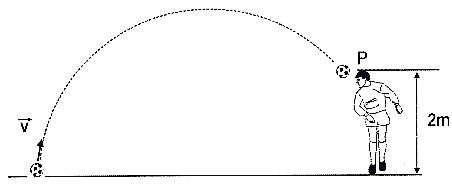
\includegraphics[height=2.9cm]{uerj_q10_tiro_de_meta}
\end{column}
\end{columns}

\alternativascurtasquatro{0}{5}{10}{15}
\end{frame}

\begin{frame}
\frametitle{Quest\~ao 10}
\framesubtitle{gabarito}
\resposta{10}{D --- 15 J}

\begin{columns}[T]
\begin{column}{0.54\textwidth}
Escolhendo o \textbf{solo} como n\'ivel zero, a energia mec\^anica se
conserva:
\[ \underbrace{\frac{m v_0^{2}}{2}}_{\text{no ch\~ao}}
   = \underbrace{E_c(P) + m g h}_{\text{no ponto P}} \]
\[ E_c(P) = \frac{0{,}5\cdot 10^{2}}{2} - 0{,}5\cdot 10\cdot 2 \]
\[ E_c(P) = 25 - 10 = \mathbf{15\ J} \]
\end{column}
\begin{column}{0.44\textwidth}
\textbf{O que \textit{n\~ao} precisou}\\
\begin{itemize}
  \item o \^angulo do chute
  \item decompor a velocidade
  \item o tempo de subida
\end{itemize}

\vspace{0.4em}
{\color{grafite}\itshape Energia \'e \textbf{escalar}. \'E por isso
que ela resolve em duas linhas o que a cinem\'atica resolveria em
seis.}
\end{column}
\end{columns}
\end{frame}

% ===================================================================
% Q13 --- UNIFOR CE
% ===================================================================
\begin{frame}
\frametitle{Quest\~ao 13}
\framesubtitle{UNIFOR CE \,\textperiodcentered\, $\sim$4 min}

\begin{columns}[T]
\begin{column}{0.60\textwidth}
Um corpo de massa $5{,}0$ kg cai verticalmente no ar, a partir do
repouso. Ap\'os percorrer $4{,}0$ m sua velocidade \'e de
$6{,}0$ m/s.

\vspace{0.4em}
Nessa queda, as mol\'eculas do corpo e do ar recebem energia que
provoca eleva\c{c}\~ao de temperatura dos corpos. De acordo com os
dados, a \textbf{energia mec\^anica perdida} pelo corpo vale, em
joules (adote $g = 10$ m/s\textsuperscript{2}):
\end{column}
\begin{column}{0.38\textwidth}
\centering
\begin{tikzpicture}[scale=1.0]
  % corpo em repouso
  \draw[thick, fill=black!8] (0.6,3.0) rectangle (1.5,3.6);
  \node[font=\small] at (1.05,3.3) {5 kg};
  \node[font=\scriptsize, anchor=west] at (1.75,3.3) {$v_0 = 0$};
  % queda
  \draw[-{Stealth[length=3mm]}, thick, black!55] (1.05,2.85) -- (1.05,1.15);
  \draw[<->] (0.15,1.0) -- (0.15,3.0)
    node[midway, left, font=\small] {$4{,}0$ m};
  % corpo embaixo
  \draw[thick, fill=black!8] (0.6,0.4) rectangle (1.5,1.0);
  \node[font=\scriptsize, anchor=west] at (1.75,0.7) {$v = 6{,}0$ m/s};
  % resist\^encia do ar: empurra para cima, contra a queda
  \draw[-{Stealth[length=2.4mm]}, thick, vinho] (0.75,1.95) -- (0.75,2.45);
  \draw[-{Stealth[length=2.4mm]}, thick, vinho] (1.35,1.95) -- (1.35,2.45);
  \node[font=\scriptsize, vinho, anchor=west, align=left] at (1.75,2.20)
    {resist\^encia\\do ar};
\end{tikzpicture}\\[0.2em]
\esquemaaula
\end{column}
\end{columns}

\alternativascurtas{110}{90}{75}{60}{45}
\end{frame}

\begin{frame}
\frametitle{Quest\~ao 13}
\framesubtitle{gabarito}
\resposta{13}{A --- 110 J}

\begin{columns}[T]
\begin{column}{0.54\textwidth}
Sempre a mesma estrutura de tr\^es linhas:
\[ E_{m_i} = E_{m_f} + E_{\text{dissipada}} \]

\[ E_{pg}\ \text{perdida} = mgh = 5\cdot 10\cdot 4 = 200\ \text{J} \]
\[ E_c\ \text{ganha} = \frac{5\cdot 6^2}{2} = 90\ \text{J} \]
\[ E_{\text{dissipada}} = 200 - 90 = \mathbf{110\ J} \]
\end{column}
\begin{column}{0.44\textwidth}
\textbf{Onde foi parar?}\\
Virou \textbf{calor} --- o corpo e o ar esquentam. A energia
n\~ao sumiu, ela \textbf{se degradou}.

\vspace{0.6em}
{\color{grafite}\itshape Confer\^encia r\'apida: sem resist\^encia do
ar a bola chegaria com $v=\sqrt{2gh}=\sqrt{80}\approx 8{,}9$ m/s. Ela
chegou com 6, ent\~ao faltou energia mesmo.}
\end{column}
\end{columns}
\end{frame}

% ===================================================================
% Q1 --- UFF
% ===================================================================
\begin{frame}
\frametitle{Quest\~ao 1}
\framesubtitle{UFF \,\textperiodcentered\, $\sim$2 min}

\linespread{0.95}\selectfont
\begin{columns}[T]
\begin{column}{0.56\textwidth}
\small
Um motorista empurra um carro sem combust\'ivel at\'e um posto mais
pr\'oximo. Na primeira metade do trajeto, ele empurra o carro
\textbf{por tr\'as} (situa\c{c}\~ao I) e na segunda metade ele o
empurra \textbf{pelo lado} (situa\c{c}\~ao II).

\vspace{0.4em}
A intensidade da for\c{c}a $\vec{F}$ \'e constante e a mesma nas duas
situa\c{c}\~oes. \'E correto afirmar que:
\end{column}
\begin{column}{0.42\textwidth}
\centering
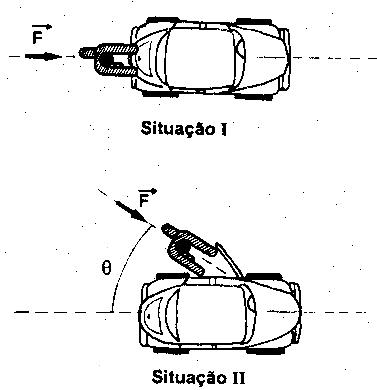
\includegraphics[height=4.3cm]{uff_q1_carro_empurrado}
\end{column}
\end{columns}

\vspace{0.1em}

\vspace{-0.3em}
{\scriptsize
\alternativascols{o trabalho realizado pelo motorista \'e maior na
situa\c{c}\~ao II.}%
{o trabalho realizado pelo motorista \'e o mesmo nas duas
situa\c{c}\~oes.}%
{a energia transferida para o carro pelo motorista \'e maior na
situa\c{c}\~ao I.}%
{a energia transferida para o carro pelo motorista \'e menor na
situa\c{c}\~ao I.}%
{o trabalho realizado na situa\c{c}\~ao I \'e menor do que a energia
transferida para o carro na situa\c{c}\~ao II.}}
\end{frame}

\begin{frame}
\frametitle{Quest\~ao 1}
\framesubtitle{gabarito}
\resposta{1}{C --- mais energia na situa\c{c}\~ao I}

\begin{columns}[T]
\begin{column}{0.54\textwidth}
\[ W = F\,d\cos\theta \]
\vspace{-1.2em}
\begin{align*}
  \text{I:}\ \ \theta = 0,\ \cos\theta = 1
    &\;\Rightarrow\; W_{\mathrm{I}} = F d\\[0.3em]
  \text{II:}\ \ \theta \neq 0,\ \cos\theta < 1
    &\;\Rightarrow\; W_{\mathrm{II}} = F d\cos\theta
\end{align*}

Mesma for\c{c}a e mesma dist\^ancia: transfere \textbf{mais} na I.
\end{column}
\begin{column}{0.42\textwidth}
\centering
\begin{tikzpicture}[scale=0.80]
  \draw[-{Stealth[length=2.6mm]}, thick] (0,0) -- (3.4,0)
    node[right, font=\small] {$d$};
  \draw[-{Stealth[length=3mm]}, very thick, vinho] (0,0) -- (2.2,0)
    node[midway, below, font=\small] {$F\cos\theta$};
  \draw[-{Stealth[length=3mm]}, very thick] (0,0) -- (2.2,1.55)
    node[midway, above, sloped, font=\small] {$\vec{F}$};
  \draw[dashed, black!45] (2.2,1.55) -- (2.2,0);
  \draw[black!70] (0.8,0) arc (0:35:0.8);
  \node[font=\small] at (0.95,0.24) {$\theta$};
\end{tikzpicture}

\vspace{0.2em}
{\color{grafite}\itshape\small S\'o a componente \textbf{na
dire\c{c}\~ao do deslocamento} faz trabalho.}
\end{column}
\end{columns}

{\color{grafite}\itshape\small A alternativa c) fala em \textbf{energia
transferida}, e n\~ao em trabalho: \'e a mesma coisa dita com outras
palavras.}
\end{frame}

% ===================================================================
% Q5 --- FGV
% ===================================================================
\begin{frame}
\frametitle{Quest\~ao 5}
\framesubtitle{FGV \,\textperiodcentered\, $\sim$4 min}

\small
Em alguns pa\'ises da Europa, os radares fotogr\'aficos das rodovias,
al\'em de detectarem a velocidade instant\^anea dos ve\'iculos, s\~ao
capazes de determinar a velocidade m\'edia desenvolvida pelos
ve\'iculos entre dois radares consecutivos.

\vspace{0.3em}
Considere dois desses radares instalados em uma rodovia retil\'inea e
horizontal. A velocidade instant\^anea de certo autom\'ovel, de
\textbf{1\,500 kg} de massa, registrada pelo primeiro radar foi de
\textbf{72 km/h}. \textbf{Um minuto depois}, o radar seguinte acusou
\textbf{90 km/h} para o mesmo autom\'ovel.

\vspace{0.3em}
O trabalho realizado pela \textbf{resultante} das for\c{c}as agentes
sobre o autom\'ovel foi, em joules, mais pr\'oximo de

\alternativascurtas{$1{,}5 \times 10^{4}$}{$5{,}2 \times 10^{4}$}%
{$7{,}5 \times 10^{4}$}{$1{,}7 \times 10^{5}$}{$3{,}2 \times 10^{5}$}
\end{frame}

\begin{frame}
\frametitle{Quest\~ao 5}
\framesubtitle{gabarito}
\resposta{5}{D --- $1{,}7\times 10^{5}$ J}

\begin{columns}[T]
\begin{column}{0.54\textwidth}
\textbf{1) Converter primeiro}
\[ 72\ \text{km/h} = 20\ \text{m/s} \qquad
   90\ \text{km/h} = 25\ \text{m/s} \]

\textbf{2) Teorema do trabalho e energia}
\[ W_{\text{total}} = \Delta E_c
   = \frac{m}{2}\left(v_f^2 - v_i^2\right) \]
\[ = \frac{1500}{2}\left(25^2 - 20^2\right) = 750\cdot 225 \]
\[ = 168\,750\ \text{J} \approx \mathbf{1{,}7\times 10^{5}\ J} \]
\end{column}
\begin{column}{0.44\textwidth}
\textbf{O distrator}\\
O \textbf{minuto} n\~ao entra na conta. Ele est\'a l\'a para quem
tenta achar a for\c{c}a e a dist\^ancia.

\vspace{0.6em}
{\color{grafite}\itshape Esta \'e a grande vantagem do teorema: liga
\textbf{velocidade} com \textbf{energia} sem precisar da for\c{c}a,
da dist\^ancia nem do tempo.}
\end{column}
\end{columns}
\end{frame}

% ===================================================================
% B\^ONUS
% ===================================================================
\begin{frame}[plain]
\vspace{1.6cm}
\centering
{\scshape\color{vinho}\Large b\^onus}\\[0.4em]
{\color{vinho}\rule{0.55\textwidth}{1.2pt}}\\[0.9em]
{\large Se sobrar tempo: Q18 (UTFPR) e Q19 (ENEM)}\\[0.4em]
{\color{grafite}\itshape as duas fecham o tema fotovoltaico}
\end{frame}

% ===================================================================
% Q18 --- UTFPR Ver\~ao 2025
% ===================================================================
\begin{frame}
\frametitle{Quest\~ao 18}
\framesubtitle{UTFPR Ver\~ao 2025 \,\textperiodcentered\, b\^onus, $\sim$2 min}

Um sistema fotovoltaico foi instalado em uma resid\^encia, com o
objetivo de amortizar a conta de energia el\'etrica.

\vspace{0.4em}
Executando uma an\'alise \textbf{ideal} (te\'orica e sem perdas), caso
for escolhido um conjunto com pot\^encia eficaz de \textbf{3\,000 W} e
considerando \textbf{8 h} de aproveitamento total da irradi\^ancia
solar por dia, quanta energia ter\'a sido gerada por este sistema no
m\^es de \textbf{setembro (30 dias)}?

\alternativascurtas{720 kWh}{720 kJ}{72 kWh}{1\,440 kWh}{1\,440 kW}
\end{frame}

\begin{frame}
\frametitle{Quest\~ao 18}
\framesubtitle{gabarito}
\resposta{18}{A --- 720 kWh}

\begin{columns}[T]
\begin{column}{0.50\textwidth}
\[ 3\,000\ \text{W} = 3\ \text{kW} \]
\[ E = P\cdot\Delta t = 3 \cdot 8 \cdot 30 \]
\[ E = \mathbf{720\ kWh} \]

\vspace{0.3em}
Sem rendimento nenhum: o enunciado diz \textbf{sem perdas}.
\end{column}
\begin{column}{0.48\textwidth}
\textbf{As alternativas testam a \textit{unidade}}
\begin{itemize}
  \item \textbf{kW} \'e pot\^encia, n\~ao energia
  \item \textbf{kJ} n\~ao sai dessa conta direta
  \item a resposta \textbf{tem} de estar em kWh
\end{itemize}

\vspace{0.4em}
{\color{grafite}\itshape Compare com a Q17: l\'a tinha rendimento de
18\%, aqui n\~ao tem nenhum. Mesma conta, uma etapa a menos.}
\end{column}
\end{columns}
\end{frame}

% ===================================================================
% Q19 --- ENEM 2015
% ===================================================================
\begin{frame}
\frametitle{Quest\~ao 19}
\framesubtitle{ENEM 2015 \,\textperiodcentered\, b\^onus, $\sim$5 min}

\small
Um carro solar \'e um ve\'iculo que utiliza apenas a energia solar para
a sua locomo\c{c}\~ao. Tipicamente, o carro cont\'em um painel
fotovoltaico que converte a energia do Sol em energia el\'etrica que,
por sua vez, alimenta um motor el\'etrico.

\vspace{0.3em}
Considere uma regi\~ao plana onde a insola\c{c}\~ao (energia solar por
unidade de tempo e de \'area que chega \`a superf\'icie da Terra) seja
de \textbf{1\,000 W/m\textsuperscript{2}}, que o carro solar possua
massa de \textbf{200 kg} e seja constru\'ido de forma que o painel
fotovoltaico em seu topo tenha uma \'area de
\textbf{$9{,}0$ m\textsuperscript{2}} e \textbf{rendimento de 30\%}.

\vspace{0.3em}
Desprezando as for\c{c}as de resist\^encia do ar, o tempo que esse
carro solar levaria, a partir do repouso, para atingir a velocidade de
\textbf{108 km/h} \'e um valor mais pr\'oximo de

\alternativascurtas{1,0 s}{4,0 s}{10 s}{33 s}{300 s}
\end{frame}

\begin{frame}
\frametitle{Quest\~ao 19}
\framesubtitle{gabarito}
\resposta{19}{D --- 33 s}

\begin{columns}[T]
\begin{column}{0.50\textwidth}
\textbf{1) Pot\^encia \'util do painel}
\[ P = 1000\cdot 9{,}0\cdot 0{,}30 = 2\,700\ \text{W} \]

\textbf{2) Energia necess\'aria}
\[ 108\ \text{km/h} = 30\ \text{m/s} \]
\[ E_c = \frac{200\cdot 30^2}{2} = 90\,000\ \text{J} \]
\end{column}
\begin{column}{0.48\textwidth}
\textbf{3) Tempo}
\[ P = \frac{E}{\Delta t} \;\Longrightarrow\;
   \Delta t = \frac{E_c}{P} \]
\[ \Delta t = \frac{90\,000}{2\,700} \approx \mathbf{33\ s} \]

\vspace{0.4em}
{\color{grafite}\itshape As tr\^es ideias da aula em uma quest\~ao
s\'o: rendimento, pot\^encia e energia cin\'etica. \'E o formato que o
ENEM mais gosta.}
\end{column}
\end{columns}
\end{frame}

% ===================================================================
% FECHAMENTO
% ===================================================================
\begin{frame}
\frametitle{O que levar da aula}
\framesubtitle{fechamento}

\begin{columns}[T]
\begin{column}{0.48\textwidth}
\textbf{As f\'ormulas}
\[ E_c = \frac{m v^2}{2} \qquad E_{pg} = mgh \]
\[ E_{pe} = \frac{k x^2}{2} \qquad W = F d\cos\theta \]
\[ \boxed{E_{m_i} = E_{m_f} + E_{\text{dissipada}}} \]
\[ W_{\text{total}} = \Delta E_c \qquad
   P = \frac{W}{\Delta t} = F v \]
\end{column}
\begin{column}{0.48\textwidth}
\textbf{Quando usar energia no lugar de $F = ma$}
\begin{itemize}
  \item Liga \textbf{velocidade com altura} e n\~ao fala em tempo
        $\Rightarrow$ \textbf{energia}
  \item Pede \textbf{for\c{c}a}, \textbf{acelera\c{c}\~ao} ou envolve
        \textbf{tempo} $\Rightarrow$ \textbf{din\^amica}
  \item Trajet\'oria curva, sem atrito $\Rightarrow$
        \textbf{energia}, porque o caminho n\~ao importa
\end{itemize}

\vspace{0.4em}
{\color{grafite}\itshape 1 kWh \'e 1 kW ligado por 1 h,\\
ou seja, $3{,}6\times10^6$ J.}
\end{column}
\end{columns}
\end{frame}

\end{document}
